\documentclass[notitlepage]{report}
\usepackage{layout}
\usepackage[a4paper, total={5in,9in}]{geometry}
\usepackage[T1]{fontenc}
\usepackage{mathtools}
\usepackage{amsthm}
\usepackage[framemethod=TikZ]{mdframed}
\usepackage{amsmath}
\usepackage{amssymb}
\usepackage{cancel}
\usepackage[dvipsnames]{xcolor}
\usepackage{tikz}
\usepackage{tikz-cd}
\usepackage{pgfplots}
\pgfplotsset{compat=1.18}
\usepackage[many]{tcolorbox}
\usepackage{import}
\usepackage{pdfpages}
\usepackage{transparent}
\usepackage{enumitem}
\usepackage[colorlinks]{hyperref}
\usepackage{csvsimple}
\usepackage{listings}
\usepackage{subcaption}
\usepackage{graphicx}
\usepackage{booktabs}

\newcommand*{\sminus}{\raisebox{1.3pt}{$\smallsetminus$}}

\newcommand*{\transp}[2][-3mu]{\ensuremath{\mskip1mu\prescript{\smash{\mathrm t\mkern#1}}{}{\mathstrut#2}}}%

% newcommand for span with langle and rangle around
\newcommand{\Span}[1]{{\left\langle#1\right\rangle}}

\newcommand{\incfig}[2][1]{%
    \def\svgwidth{#1\columnwidth}
    \import{./figures/}{#2.pdf_tex}
}

\pdfsuppresswarningpagegroup=1

\newcounter{theo}[section]\setcounter{theo}{0}
\renewcommand{\thetheo}{\arabic{section}.\arabic{theo}}

\newcounter{excounter}[section]\setcounter{excounter}{0}
\renewcommand{\theexcounter}{\arabic{section}.\arabic{excounter}}

\numberwithin{equation}{section}

\newenvironment{theorem}[1][]{
    \refstepcounter{theo}
     \ifstrempty{#1}
    {\mdfsetup{
        frametitle={
            \tikz[baseline=(current bounding box.east),outer sep=0pt]
            \node[anchor=east,rectangle,fill=blue!20,rounded corners=5pt]
            {\strut Teorema~\thetheo};}
        }
    }{\mdfsetup{
        frametitle={
            \tikz[baseline=(current bounding box.east),outer sep=0pt]
            \node[anchor=east,rectangle,fill=blue!20,rounded corners=5pt]
            {\strut Teorema~\thetheo:~#1};}
        }
    }
    \mdfsetup{
        roundcorner=10pt,
        innertopmargin=10pt,linecolor=blue!20,
        linewidth=2pt,topline=true,
        frametitleaboveskip=\dimexpr-\ht\strutbox\relax,
        % nobreak=false
    }
\begin{mdframed}[]\relax}{
\end{mdframed}}
\newtcolorbox[auto counter, number within=section]{definition}[2][]{
    colframe=violet!0,
    coltitle=violet, % Title text color
    fonttitle=\bfseries, % Title font
    title={Definizione~\thetcbcounter:~#2}, % Title format
    sharp corners, % Less rounded corners
    boxrule=0pt, % Line width of the box frame
    toptitle=1mm, % Distance from top to title
    bottomtitle=1mm, % Distance from title to box content
    colbacktitle=violet!5, % Background color of the title bar
    left=0mm, right=0mm, top=1mm, bottom=1mm, % Padding around content
    enhanced, % Enable advanced options
    before skip=10pt, % Space before the box
    after skip=10pt, % Space after the box
    breakable, % Allow box to split across pages
    colback=violet!0,
    borderline west={2pt}{-5pt}{violet!40},
    #1
}

\newenvironment{lemmao}[1][]{
    \refstepcounter{theo}
     \ifstrempty{#1}
    {\mdfsetup{
        frametitle={
            \tikz[baseline=(current bounding box.east),outer sep=0pt]
            \node[anchor=east,rectangle,fill=green!20,rounded corners=5pt]
            {\strut Lemma~\thetheo};}
        }
    }{\mdfsetup{
        frametitle={
            \tikz[baseline=(current bounding box.east),outer sep=0pt]
            \node[anchor=east,rectangle,fill=green!20,rounded corners=5pt]
            {\strut Lemma~\thetheo:~#1};}
        }
    }
    \mdfsetup{
        roundcorner=10pt,
        innertopmargin=10pt,linecolor=green!20,
        linewidth=2pt,topline=true,
        frametitleaboveskip=\dimexpr-\ht\strutbox\relax,
        % nobreak=true
    }
\begin{mdframed}[]\relax}{
\end{mdframed}}

\theoremstyle{plain}
\newtheorem{lemma}[theo]{Lemma}
\newtheorem{corollary}{Corollario}[theo]
\newtheorem{proposition}[theo]{Proposizione}

\theoremstyle{definition}
\newtheorem{example}[excounter]{Esempio}

\theoremstyle{remark}
\newtheorem*{note}{Nota}
\newtheorem*{remark}{Osservazione}

\newtcolorbox{notebox}{
  colback=gray!10,
  colframe=black,
  arc=5pt,
  boxrule=1pt,
  left=15pt,
  right=15pt,
  top=15pt,
  bottom=15pt,
}

\DeclareRobustCommand{\rchi}{{\mathpalette\irchi\relax}} % beautiful chi
\newcommand{\irchi}[2]{\raisebox{\depth}{$#1\chi$}} % inner command, used by \rchi
\newtcolorbox[auto counter, number within=section]{eser}[1][]{
    colframe=black!0,
    coltitle=black!70, % Title text color
    fonttitle=\bfseries\sffamily, % Title font
    title={Esercizio~\thetcbcounter~#1}, % Title format
    sharp corners, % Less rounded corners
    boxrule=0pt, % Line width of the box frame
    toptitle=1mm, % Distance from top to title
    bottomtitle=1mm, % Distance from title to box content
    colbacktitle=black!5, % Background color of the title bar
    left=0mm, right=0mm, top=1mm, bottom=1mm, % Padding around content
    enhanced, % Enable advanced options
    before skip=10pt, % Space before the box
    after skip=10pt, % Space after the box
    breakable, % Allow box to split across pages
    colback=black!0,
    borderline west={1pt}{-5pt}{black!70},
}
\newcommand{\seminorm}[1]{\left\lvert\hspace{-1 pt}\left\lvert\hspace{-1 pt}\left\lvert#1\right\lvert\hspace{-1 pt}\right\lvert\hspace{-1 pt}\right\lvert}

\definecolor{codegreen}{rgb}{0,0.6,0}
\definecolor{codegray}{rgb}{0.5,0.5,0.5}
\definecolor{codepurple}{rgb}{0.58,0,0.82}
\definecolor{backcolour}{rgb}{0.95,0.95,0.92}
\lstdefinestyle{mystyle}{
    backgroundcolor=\color{backcolour},   
    commentstyle=\color{codegreen},
    keywordstyle=\color{magenta},
    numberstyle=\tiny\color{codegray},
    stringstyle=\color{codepurple},
    basicstyle=\ttfamily\footnotesize,
    breakatwhitespace=false,         
    breaklines=true,                 
    captionpos=b,                    
    keepspaces=true,                 
    numbers=left,                    
    numbersep=5pt,                  
    showspaces=false,                
    showstringspaces=false,
    showtabs=false,                  
    tabsize=2
}

\lstset{style=mystyle}

\title{Report Lab 2\\\small Experimental Physics for AI 2}
\author{Doğa Tekeli, Osea Fracchia, \\ Carlotta Maria Portinaro, Gabriele
Roberto Bovo}
\date{First semester 2024 \-- 2025}

\begin{document}
\maketitle

\begin{abstract}
The study examines the potential differences across resistors and capacitors in
RC circuits, and across resistors and inductors in RL circuits using an
oscilloscope and deriving and validating time constants for these systems. The
same setup is then used to study RLC circuits. These
procedures help understanding the study of time-dependent circuit dynamics.
\end{abstract}

\chapter{Study of RC and RL circuits in pulsed current }

\section{Goal}
We will study the behavior of RC and RL circuits in response to pulsed current generated by a square-wave signal. 

Specifically, analyzing the potential differences across the resistor and capacitance (RC Circuit) and across the resistor and inductance (RL circuit). 

Since we know the resistances of each experiment, we will calculate the time constant for the circuits given the formulas, for the RC circuit:
\[
\tau = R \cdot C
\]

where \( \tau \) is the time constant in seconds,  \( R \) is the resistance in ohms, \( \Omega \) and \( C \) is the capacitance in farads, \( F \).



For the RL circuit:
\[
\tau = \frac{L}{R}
\]

where \( \tau \) is the time constant in seconds,  \( R \) is the resistance in ohms, \( \Omega \) and \( L \) is the inductance in henrys, \( H \).

\section{Method}
We will use an oscilloscope to measure the time-varying voltage signals. 

\begin{figure}
    \centering
    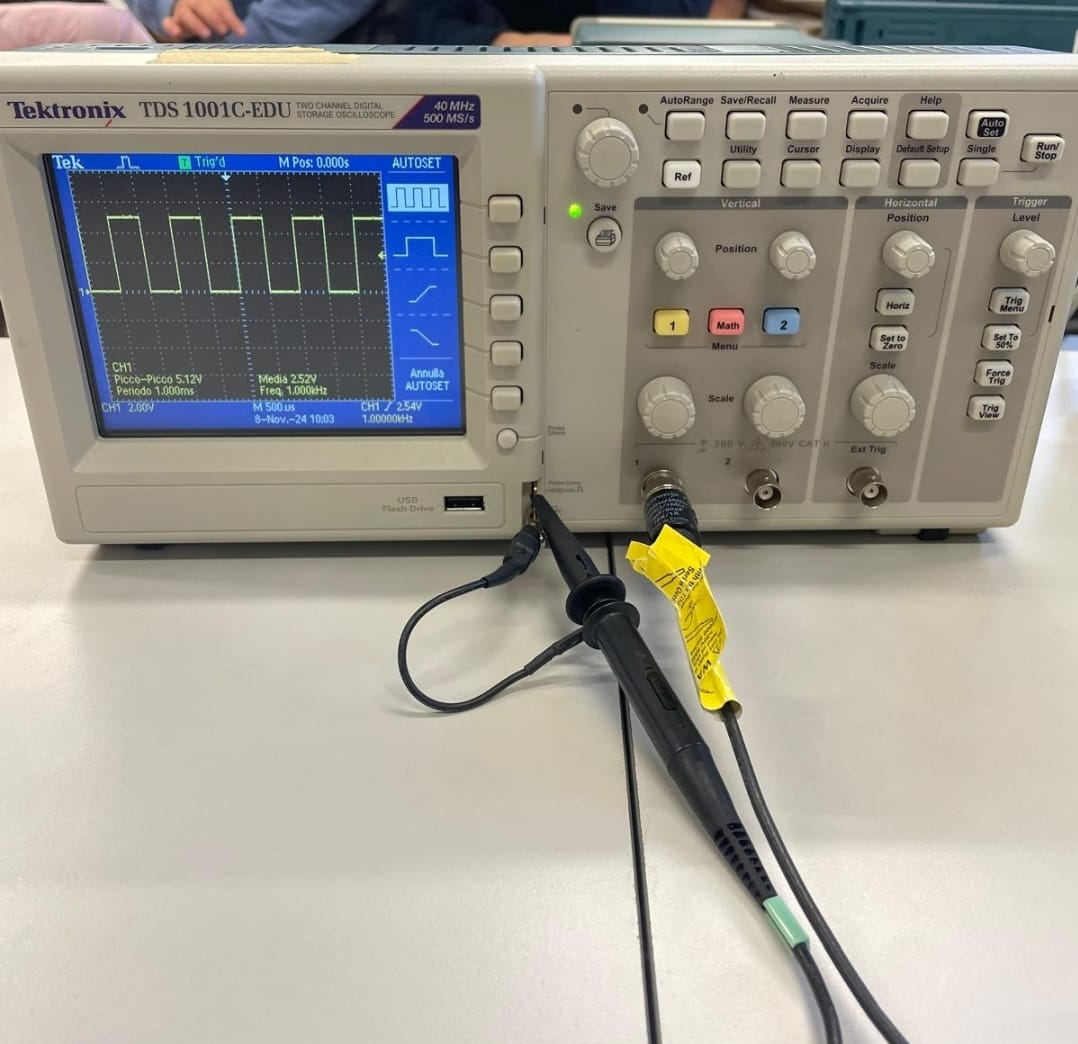
\includegraphics[width=0.5\linewidth]{figures/probes_test.jpeg}
    \caption{The testing of the probes}
    \label{fig:probes_test}
\end{figure}


Before connecting the probes to our actual circuits, we check the probe compensation by connecting the probes to the test points in our oscilloscope. It is seen in figure~\ref{fig:probes_test} that the probes are correctly calibrated and therefore result in a square wave.

Then, we configure the RC circuit, the resistor and the capacitor are connected in series as seen in figure~\ref{fig:setup-rc} with a square-wave signal generated by a function generator. We record the voltage waveforms during both the capacitor’s charge and discharge phases with a voltage generator (battery) at frequency  \( f \)=1400 \( Hz \), constant capacitance \(C\) and with different resistances.

We apply a similar procedure for the RL circuit at frequency \( f \)=500 \( Hz \) and by keeping the inductance L as constant.


\begin{figure}
    \centering
    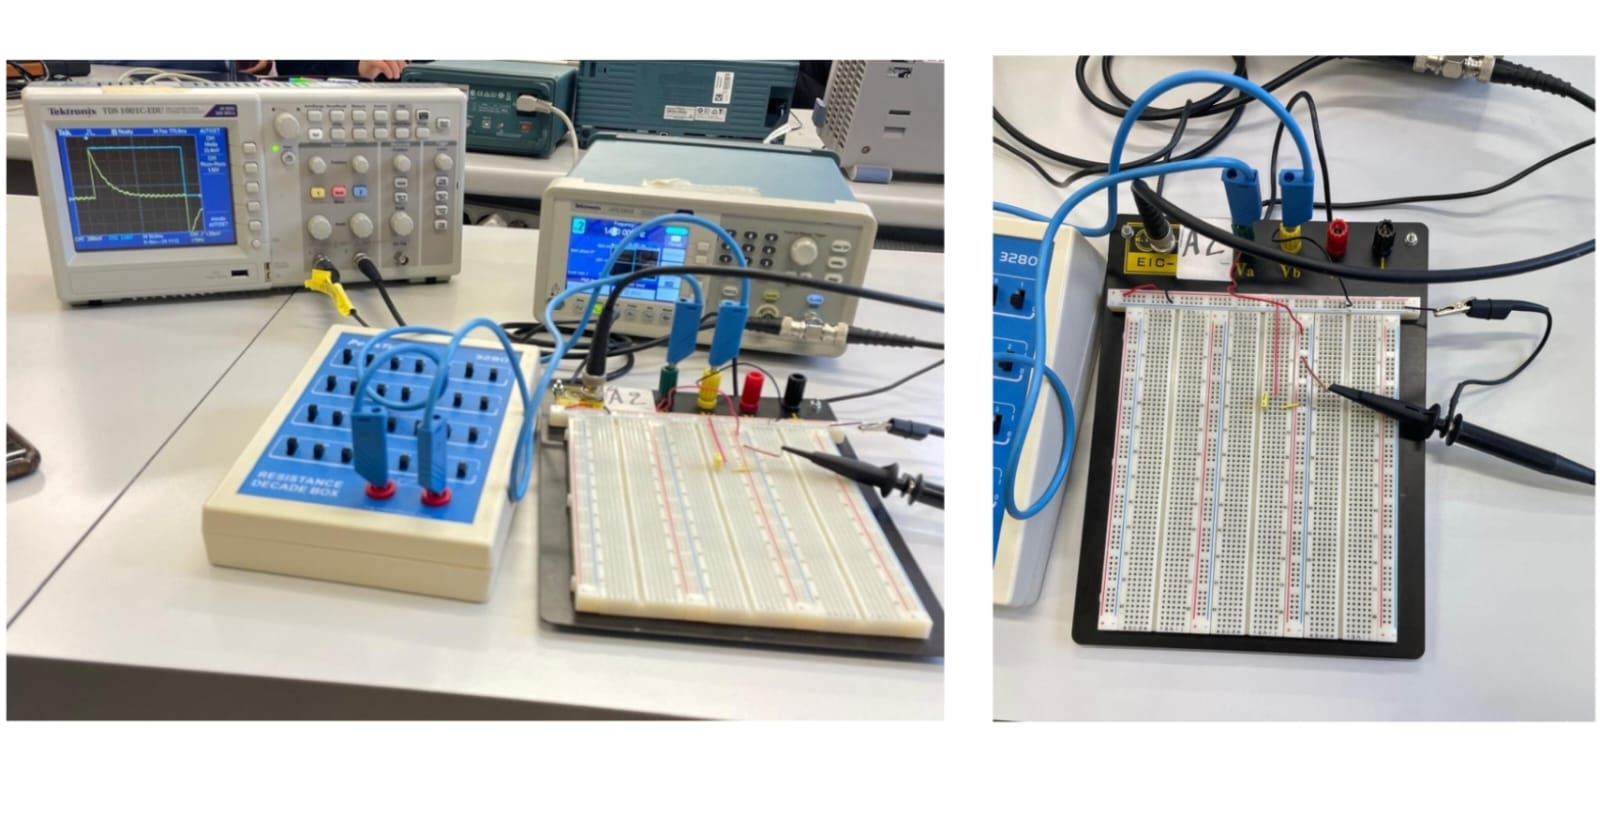
\includegraphics[width=1\linewidth]{figures/RC_pictures.jpeg}
    \caption{RC setup of the experiment}
    \label{fig:setup-rc}
\end{figure}


\section{Data}  

In the manual, the TBS1000B Digital Storage Oscilloscope has its vertical accuracy specified as:

\[
\pm \left(3\% \times \text{reading} + 0.2 \text{ div} + 1 \, \text{mV}\right),
\]

where the division size (\textit{div}) depended on the selected vertical scale. The horizontal time base accuracy was:

\[
\pm 50 \, \text{ppm} \times \text{time measurement}.
\]


   \section{Analysis}

   \subsection{The behavior of RC circuits}

During the charging phase in RC circuits, when the circuit is closed with a voltage generator, the capacitor voltage \( V_C(t) \) increases exponentially as:
        \[
        V_C(t) = V \left(1 - e^{-t / \tau}\right), \quad \text{where} \ \tau = RC \ \text{is the time constant.}
        \]
        The current \( I(t) \) decreases as:
        \[
        I(t) = \frac{V}{R} e^{-t / \tau}.
        \]
        During the discharging phase, when the circuit is closed on a short circuit, the capacitor voltage \( V_C(t) \) decreases exponentially as:
        \[
        V_C(t) = V_C(0) e^{-t / \tau}.
        \]
        Similarly, the current \( I(t) \) becomes:
        \[
        I(t) = -\frac{V_C(0)}{R} e^{-t / \tau}.
        \]
        The behavior when the polarity of the generator voltage is reversed, causes the capacitor to first discharge and then recharge in the opposite polarity:
        \[
        V_C(t) = -V \left(1 - e^{-t / \tau}\right).
        \]
    \subsection{The behavior of RL circuits}
    Here, we analyze the charging and discharging phases of an RL circuit:
During the charging phase, when the circuit is closed with a voltage generator, the current \( I(t) \) increases exponentially as:
        \[
        I(t) = \frac{V}{R} \left(1 - e^{-t / \tau}\right), \quad \text{where} \ \tau = \frac{L}{R} \ \text{is the time constant.}
        \]
        meanwhile during the discharging phase, when the circuit is closed on a short circuit, the current \( I(t) \) decreases exponentially as:
        \[
        I(t) = I(0) e^{-t / \tau}.
        \]
        The behavior when the polarity of the generator voltage is reversed, causes the current to reverse the direction as before.
        \[
        I(t) = -\frac{V}{R} \left(1 - e^{-t / \tau}\right).
        \]
\subsection{Oscilloscope Graphs of the RC Circuit}

To study the charging and discharging behavior of an RC circuit, we conducted experiments with varying resistances (\(R\)) while maintaining a voltage generator with a fixed frequency of \(1400 \, \text{Hz}\). The resistances used in the experiment were \(1 \, \text{M}\Omega\), \(2 \, \text{M}\Omega\), \(5 \, \text{M}\Omega\), and \(10 \, \text{M}\Omega\). After setting the horizontal time scale and vertical voltage scale, corresponding oscilloscope readings are shown in Figures~\ref{fig:RC_1}, \ref{fig:RC_2}, \ref{fig:RC_3}, and \ref{fig:RC_4}.

As the resistance increases the time constant of the circuit, \(\tau = RC\), increases, leading to a slower charging and discharging process. The voltage across the capacitor (\(V_C\)) reaches steady-state values more gradually for higher resistances. The exponential nature of the charging and discharging curves is seen in the cases.

The following figures display the oscilloscope traces for different resistance values:
\begin{figure}[h!]
    \centering
    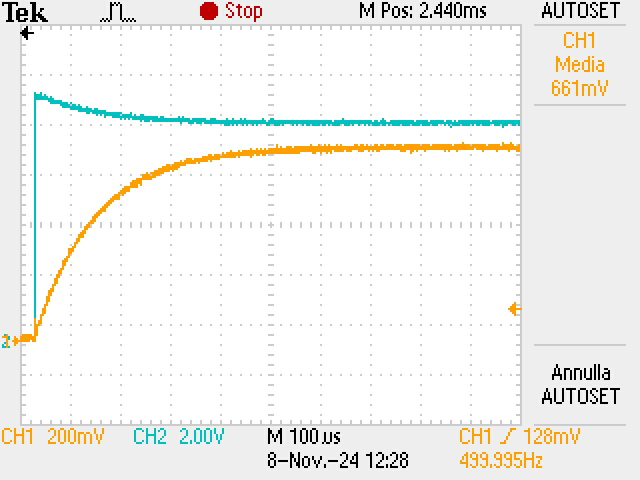
\includegraphics[width=0.4\linewidth]{figures/RC_graph_1.JPG}
    \caption{RC Circuit behavior with \(R = 10 \, \text{M}\Omega\)}
    \label{fig:RC_1}
\end{figure}

\begin{figure}[h!]
    \centering
    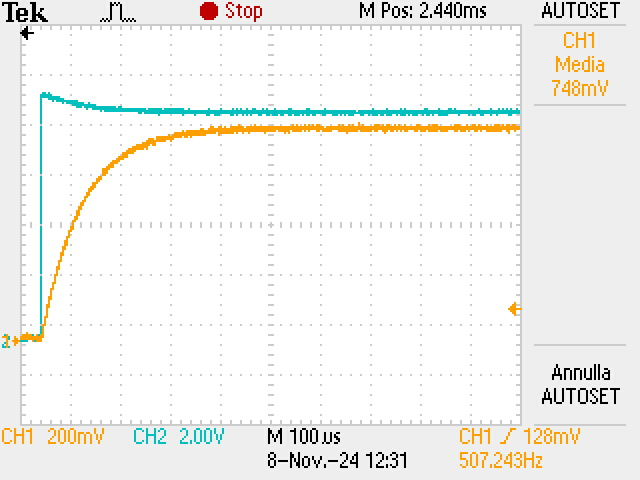
\includegraphics[width=0.4\linewidth]{figures/RC_graph_2.JPG}
    \caption{RC Circuit behavior with \(R = 5 \, \text{M}\Omega\)}
    \label{fig:RC_2}
\end{figure}

\begin{figure}[h!]
    \centering
    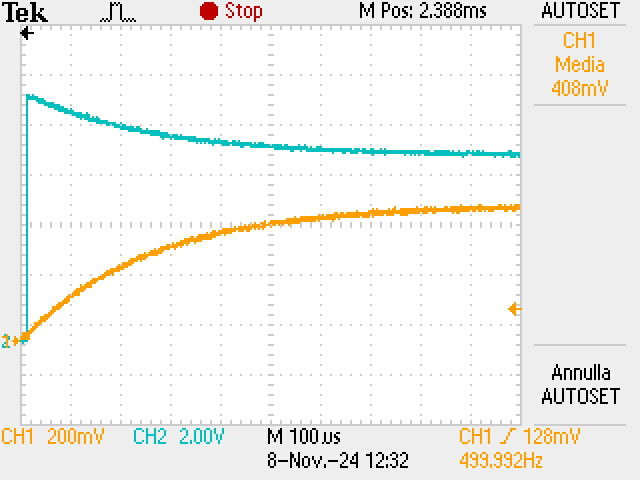
\includegraphics[width=0.4\linewidth]{figures/RC_graph_3.JPG}
    \caption{RC Circuit behavior with \(R = 2 \, \text{M}\Omega\)}
    \label{fig:RC_3}
\end{figure}

\begin{figure}[h!]
    \centering
    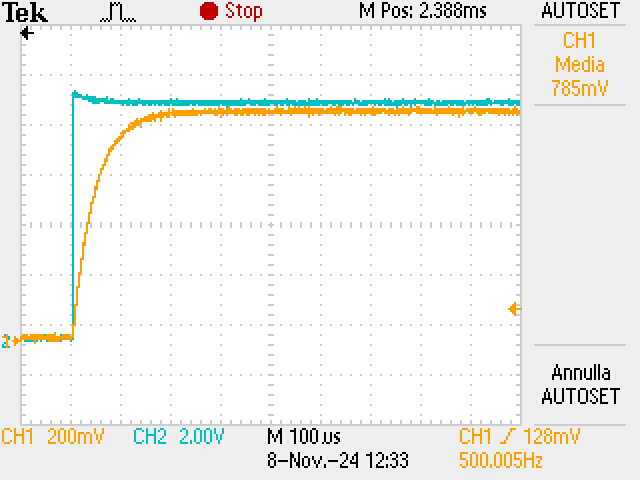
\includegraphics[width=0.4\linewidth]{figures/RC_graph_4.JPG}
    \caption{RC Circuit behavior with \(R = 1 \, \text{M}\Omega\)}
    \label{fig:RC_4}
\end{figure}

\section*{Estimating the Capacitance of an RC Circuit}

We have seen earlier that in an RC charging circuit, the voltage across the capacitor \( V(t) \) follows the exponential law:
\[
V(t) = V_{\text{max}} \left( 1 - e^{-t / \tau} \right),
\]

At \( t = \tau \), the voltage reaches approximately \( 63\% \) of \( V_{\text{max}} \) since \( e^{-1} \approx 0.37 \).

In the graph \ref{fig:RC_1}, we are given an RC circuit where the oscilloscope shows that the capacitor voltage reaches approximately \( V_{\text{max}} \) after 5 horizontal divisions, with the total time duration spanning approximately 10 seconds.

From this information, the time constant \( \tau \), corresponding to one-fifth of the total time (as the capacitor charges to \( V_{\text{max}} \) after approximately 5 time constants), is given by:  
\[
\tau = \frac{\text{Total time}}{5} = \frac{10 \, \text{s}}{5} = 2 \, \text{s}.
\]

The time constant \( \tau \) is related to the resistance \( R \) and the capacitance \( C \) of the RC circuit by the formula:  
\[
\tau = R \times C
\]

Substituting the known value of \( \tau = 2 \, \text{s} \) and the resistance \( R = 10 \, \text{M}\Omega = 10^7 \, \Omega \):  
\[
C = \frac{\tau}{R} = \frac{2 \, \text{s}}{10^7 \, \Omega} = 2 \times 10^{-7} \, \text{F} = 0.2 \, \mu\text{F}
\]

Thus, the estimated capacitance of the circuit is:  
\[
C \approx 0.2 \, \mu\text{F}
\]

    \subsection{Oscilloscope Graphs of the RL Circuit}
To study the behavior of an RL circuit, we conducted experiments using varying resistances (\(R\)) while maintaining a voltage generator with a fixed frequency of \(500 \, \text{Hz}\). The resistances used in the experiment were \(100 \, \Omega\), \(300 \, \Omega\), \(500 \, \Omega\), and \(1000 \, \Omega\). After configuring the horizontal time scale and vertical voltage scale, the oscilloscope readings are presented in Figures~\ref{fig:RL_1}, \ref{fig:RL_2}, \ref{fig:RL_3}, and \ref{fig:RL_4}.

As the resistance increases, the time constant of the RL circuit, \(\tau = \frac{L}{R}\), decreases, resulting in a faster rise and decay of the current. This is reflected in the steeper exponential curves observed for higher resistance values. The voltage across the inductor (\(V_L\)) demonstrates the transient behavior expected in an RL circuit. In figure \ref{fig:RL_3} since the resistance is small, it can be seen that the inductor opposes rapid changes in current more significantly.

The following figures display the oscilloscope traces for different resistance values:

\begin{figure}[h!]
    \centering
    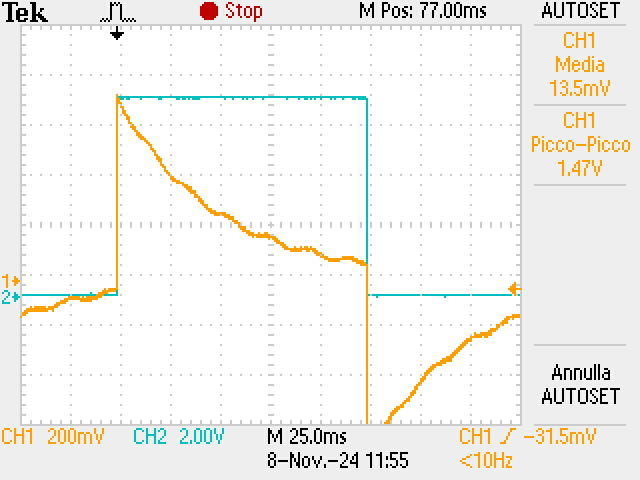
\includegraphics[width=0.4\linewidth]{figures/RL_graph_4.JPG}
    \caption{RL Circuit behavior with \(R = 100 \, \Omega\)}
    \label{fig:RL_3}
\end{figure}

\begin{figure}[h!]
    \centering
    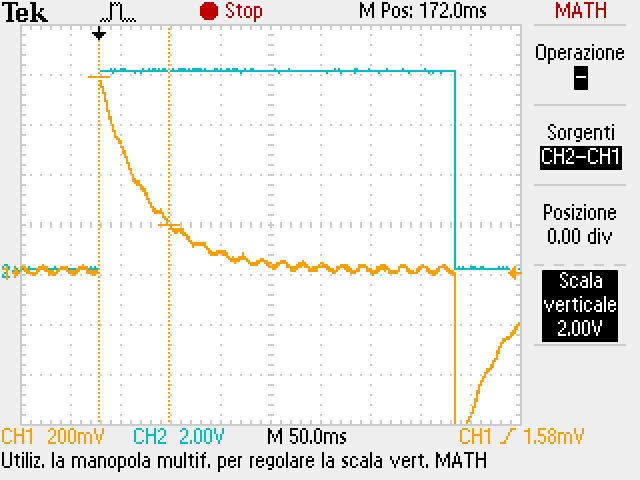
\includegraphics[width=0.4\linewidth]{figures/RL_graph_1.JPG}
    \caption{RL Circuit behavior with \(R = 300 \, \Omega\)}
    \label{fig:RL_1}
\end{figure}

\begin{figure}[h!]
    \centering
    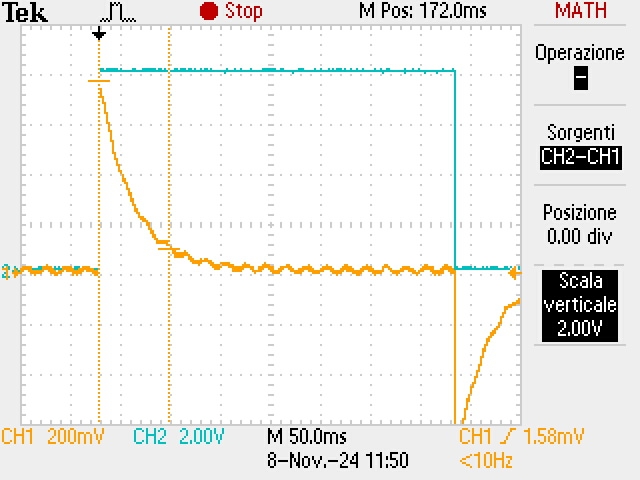
\includegraphics[width=0.4\linewidth]{figures/RL_graph_2.JPG}
    \caption{RL Circuit behavior with \(R = 500 \, \Omega\)}
    \label{fig:RL_2}
\end{figure}

\begin{figure}[h!]
    \centering
    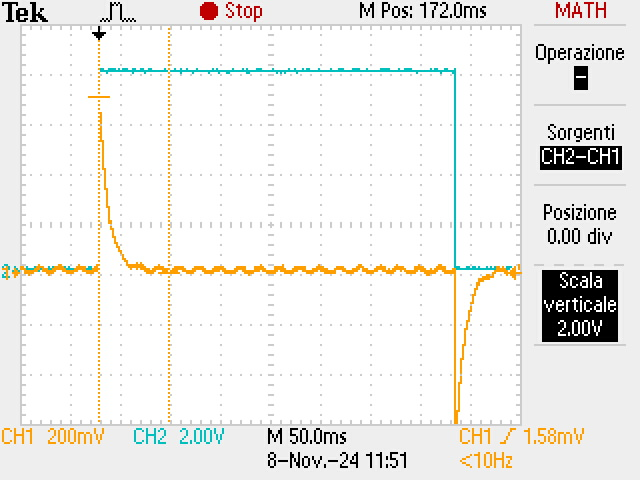
\includegraphics[width=0.4\linewidth]{figures/RL_graph_3.JPG}
    \caption{RL Circuit behavior with \(R = 1000 \, \Omega\)}
    \label{fig:RL_4}
\end{figure}

\section*{Estimating the Inductance of an RL Circuit}

Let's use figure~\ref{fig:RL_4} with \( R = 1000 \, \Omega \) where \( \tau \) is defined as before:
\[
\tau = \frac{L}{R}
\]

At \( t = \tau \), the current reaches approximately \( 63\% \) of \( I_{\text{max}} \) since \( e^{-1} \approx 0.37 \).

In the graph, we observe an RL circuit with a resistance \( R = 1000 \, \Omega \). The oscilloscope indicates that the current reaches \( 63\% \) of \( I_{\text{max}} \) after approximately 2 horizontal divisions, let's assume the time for one division corresponds to \( 1 \, \text{ms} \). Therefore, the time constant becomes:
\[
\tau = 2 \, \text{divisions} \times 1 \, \text{ms/division} = 2 \, \text{ms}
\]

Using the relationship between the time constant, resistance, and inductance:
\[
L = \tau \cdot R
\]
Substituting \( \tau = 2 \, \text{ms} = 2 \times 10^{-3} \, \text{s} \) and \( R = 1000 \, \Omega \):
\[
L  \approx  \ 2 \times 10^{-3} \, \text{s} \cdot 1000 \, \Omega = 2 \, \text{H}
\]


\chapter{Study of RLC circuits in pulsed current}


\section{Goal}
In this part of the experiment, our main goal is to study the trend of potential difference at the ends of each part of the RLC circuit stressed by a square-wave signal. Based on the observed waveform, we had to determine the period of the oscillations in the different regimes and compare it to the formula varying $R$.

\section{Setup}
The setup of the RLC circuit is shown in figure~\ref{fig:setup-rlc}. The circuit
consists of a resistor, inductor, and capacitor connected in series. The
square-wave signal generated by the function generator is applied to the
circuit. One probe of the oscilloscope is used to measure the voltage signals at
the ends of the resistor, inductor, and capacitor, and the other probe at the
ends of the resistor only.

\begin{figure}[h!]
    \centering
    \begin{subfigure}[h]{0.45\textwidth}
        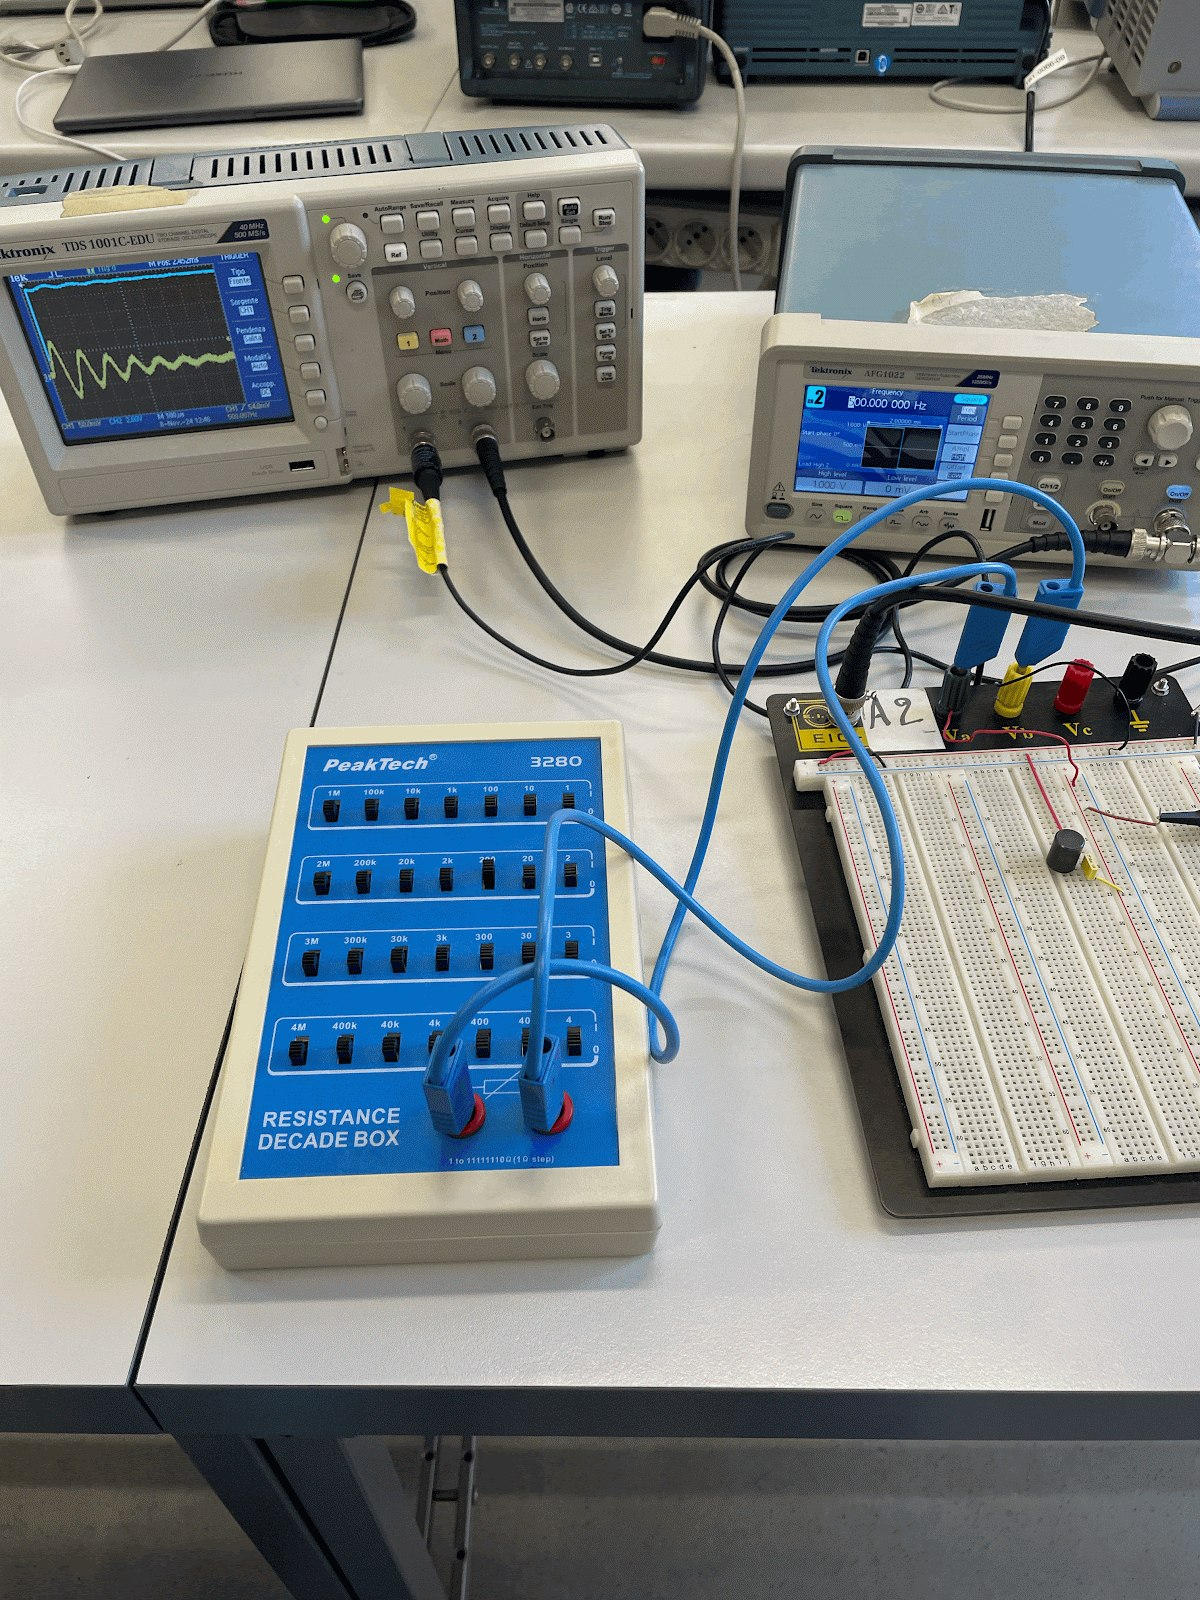
\includegraphics[width=\textwidth]{figures/RLC_setup_1.jpg}\caption{}\label{fig:setup1.21}
    \end{subfigure}
    \begin{subfigure}[h]{0.45\textwidth}
        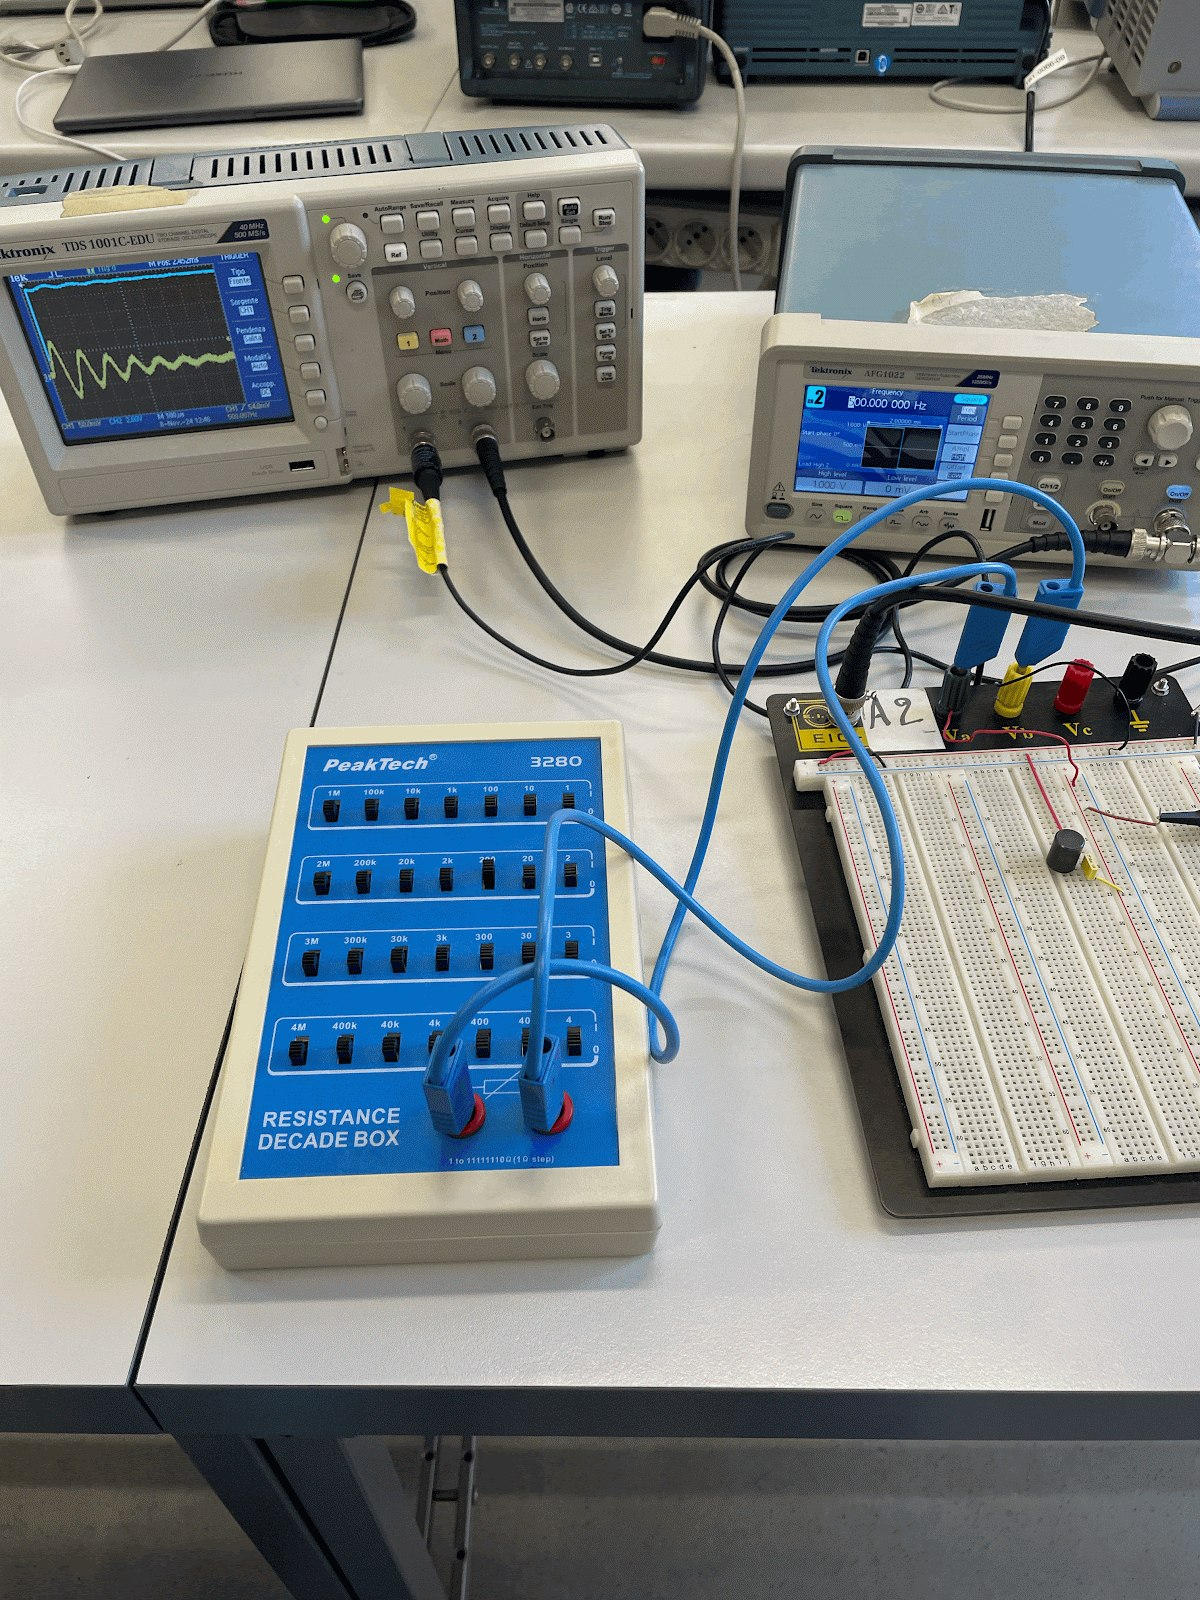
\includegraphics[width=\textwidth]{figures/RLC_setup_2.jpg}\caption{}\label{fig:setup1.22}
    \end{subfigure}
    \begin{subfigure}[h]{\textwidth}
        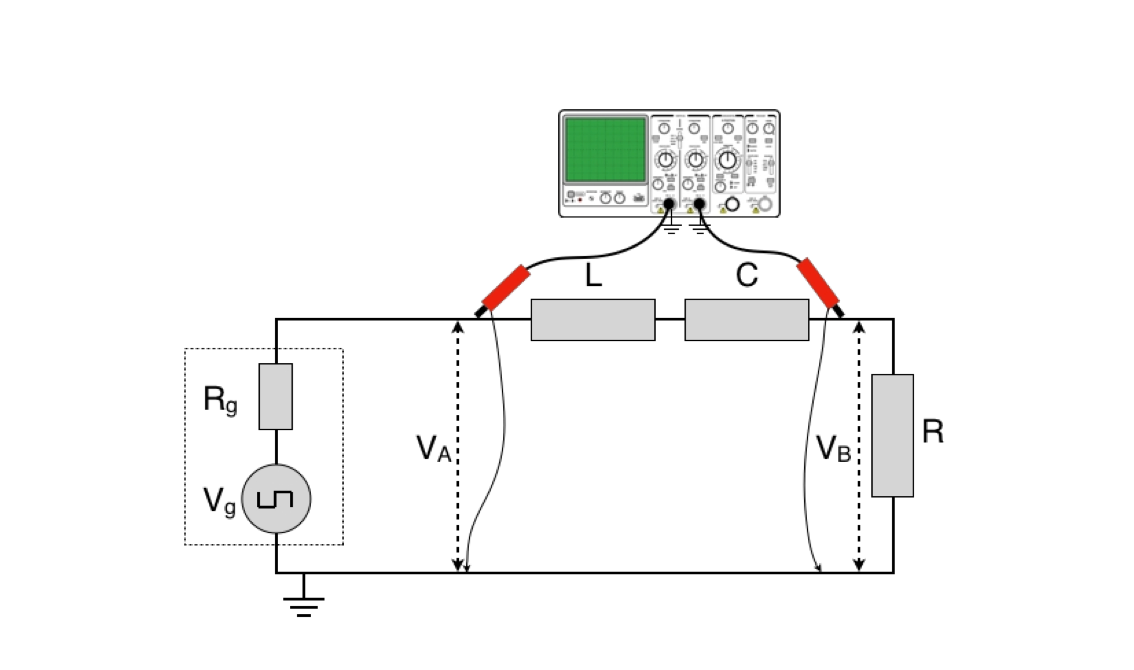
\includegraphics[width=\textwidth]{figures/diagram_RLC.png}\caption{}\label{fig:setup1.diag}
    \end{subfigure}
    \caption{Setup of the experiment}\label{fig:setup-rlc}
\end{figure}


\section{Method}
Once we constructed the RLC circuit (image~\ref{fig:setup1.21}), a function
generator was used
to produce a square-wave signal of frequency $f = 500$ Hz. Using an
oscilloscope, we measured each voltage signal at the ends of the different $R$
chosen, using a probe.

We calibrated the channels of the screen of the oscilloscope so that the third
maximum of \(VR{(t)}\) si no less than $\frac{1}{10}$ of the first and the
frequency of the square wave such that at least 5 local maxima are seen. Instead
for critically damped and overdamped circuits, we set the frequency of the
square wave such that \(VR{(t)}\) can be seen reduced to at least $\frac{1}{10}$
of its value. To visualize at best the waves we fixed the channels at \(CH1 =
50.0 mV\) and \(CH2 = 2.00 V\) 

It is possible to observe two distinct lines that represent the two channels,
\(CH1\) and \(CH2\) that are: the orange one (\(CH1\)) is the behavior of the
circuit, while the second channel \(CH2\) is the tension entering circuit.

\section{Analysis}
\subsection{Behavior of RLC}
The RLC circuit is made of three components:
\begin{itemize}
    \item Resistor (\(R\)): Dissipates energy as heat.
    \item Inductor (\(L\)): Stores energy in its magnetic field.
    \item Capacitor (\(C\)): Stores energy in its electric field.
\end{itemize}

The governing equation for the RLC circuit can be derived using Kirchhoff's
Voltage Law:
\[ V_R + V_L + V_C = 0 \implies  L\frac{d^2q}{dt^2} + R\frac{dq}{dt} + \frac{q}{C} = 0 \]

When we have a damped oscillator, the general solution is:
\[
  q{(t)} = Q_{0} e^{-\alpha t} \cos{(w_d t + \phi)}
\]
where 
\begin{itemize}[label = --]
    \item \(\alpha = \frac{R}{2L}\) is the damping term
    \item \(W_d = {\left( \frac{1}{LC} - {\left( \frac{R}{LC} \right)} ^2
        \right)}^{\frac{1}{2}} \) is the damped angular frequency
    \item \(Q_{0}\) is the initial charge on the capacitor
\end{itemize}
The period in the RLC circuit is found as:
\[
    T = \frac{2\pi}{w_d} = \frac{1}{f}
\]
\subsection{Underdamped case}
In an underdamped circuit, the capacitor discharges because the energy
oscillates between the capacitor and the inductor while gradually being lost as
heat in the resistor. The resistance must be
\[
    R < \sqrt{\frac{4L}{C}}
\]

\begin{figure}[h!]
    \centering
    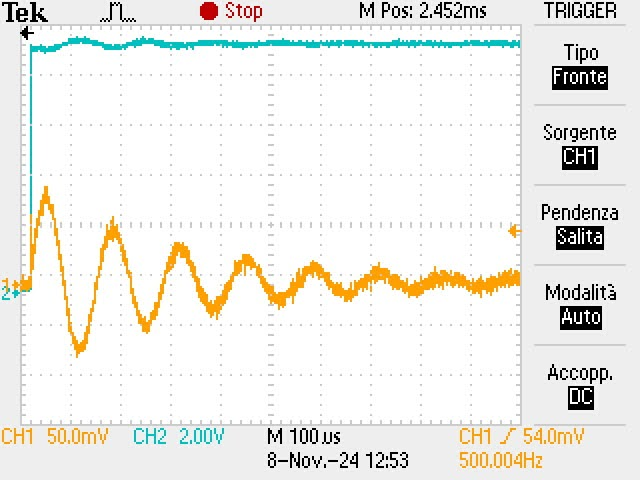
\includegraphics[width=0.45\linewidth]{figures/RLC_graph_1.jpg}
    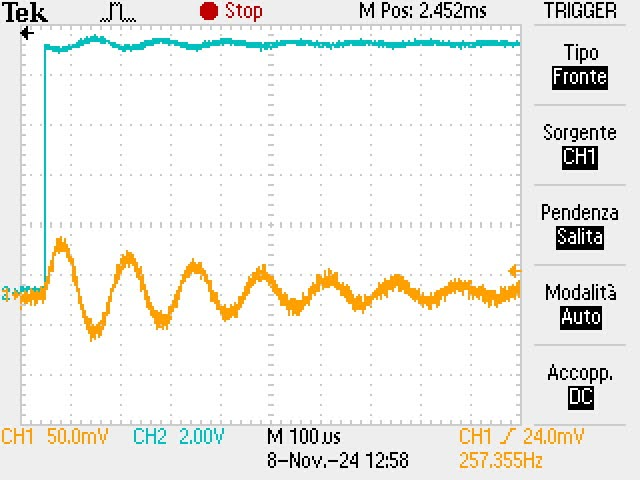
\includegraphics[width=0.45\linewidth]{figures/RLC_graph_2.jpg}
    \caption{Underdamped RLC circuit}\label{fig:underdamped}
\end{figure}

For both pictures in figure~\ref{fig:underdamped} we have an underdamped
circuit, the period we can calculate from \(T = \frac{1}{f}\) is 
\[
  T_{1} = \frac{1}{500.004 Hz} = 0.0019s \quad \quad T_{2} = \frac{1}{257.355
  Hz} = 4 ms
\]

Instead of calculating the period from the images we have to multiply the number
of divisions with the time per division. In~\ref{fig:underdamped} left
specifically we have:
\[
  T_{1} = 2 \text{ divisions } \cdot 100
  \frac{\text{microseconds}}{\text{divisions}} = 200 \mu s = 0.0002 s
\]

while for the right image we have:
\[
  T_{2} = 3.9 \text{ divisions } \cdot 100
  \frac{\text{microseconds}}{\text{divisions}} = 390 \mu s = 0.00039 s
\]

\subsection{Overdamped case}
In an overdamped circuit, the resistor dominates, and the oscillations are
suppressed, leading to a monotonic decay of charge and current, and we get a
fast decay without oscillations. The resistance must be
\[
  R > \sqrt{\frac{4L}{C}}
\]
\begin{figure}[h!]
    \centering
    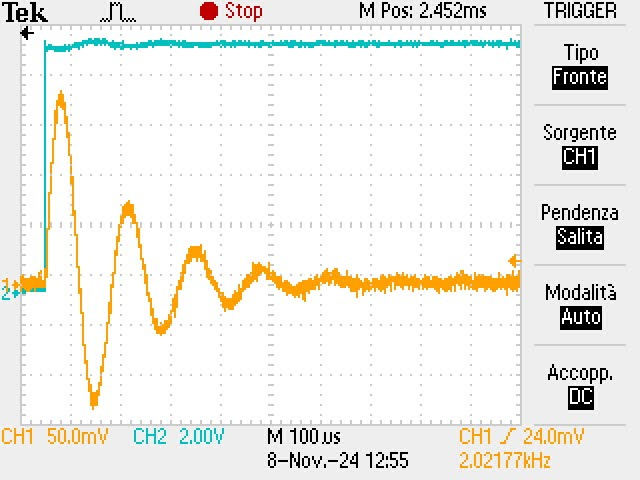
\includegraphics[width=0.45\linewidth]{figures/RLC_graph_3.jpg}
    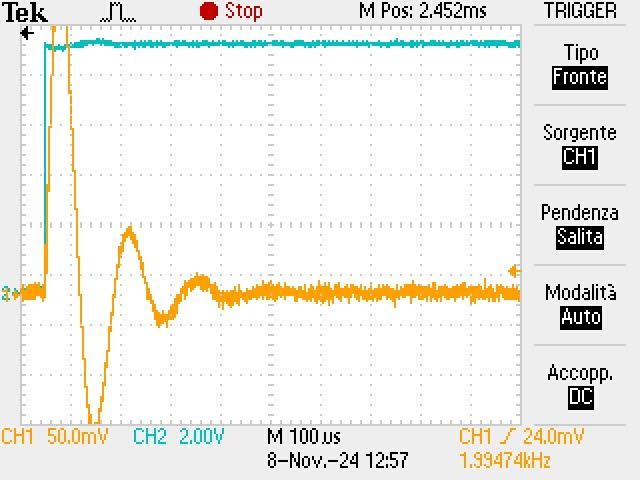
\includegraphics[width=0.45\linewidth]{figures/RLC_graph_4.jpg}
    \caption{Overdamped RLC circuit}\label{fig:overdamped}
\end{figure}

Pictures in figure~\ref{fig:overdamped} show an overdamped circuit, the period
we can enumerate is
\[
  T_{3} = \frac{1}{2.02177 \cdot 10^{3} Hz} = 5\cdot 10^{-4} s \quad \quad T_{4}=
  \frac{1}{1.99474 \cdot 10^{3} Hz} = 5\cdot 10^{-4}s
\]
Alternatively, the period from the images can be found by multiplying the number
of divisions by the time per division. In the left image of~\ref{fig:overdamped}
specifically we have that
\[
    T_{3} = 5 \text{ divisions } \cdot  100
    \frac{\text{microseconds}}{\text{divisions}} = 500 \mu s = 0.0005 s
\]
while for the right image we have that
\[
    T_{4} = 5.2 \text{ divisions } \cdot  100
    \frac{\text{microseconds}}{\text{divisions}} = 520 \mu s = 0.00052 s
\]

\subsection{Critically damped case}
In a critically damped circuit, we have the same state as for the overdamped one
but we get a slow decay without oscillations. The resistor must be
\[
    R = R_C = \sqrt{\frac{4L}{C}}
\]
We didn't observe any critical dumping in our analysis.

\section{Conclusions}

We studied the trend of the potential difference at the end of the resistor, the
inductance and the conductor of our RLC circuit stressed by a square-wave
signal.

Then we determined the period of the oscillations in the different regimes that
we observed on the oscilloscope and we compared it to the one calculated from
the theory. We noticed that for the underdamped circuit in
figure~\ref{fig:underdamped} we have a dismatch in the two results. Instead for
the overdamped circuit the results are consistent.
\end{document}
